% =============================================================================
%  T1 / P1 - Limiarizacao de imagens e video
%  Processamento de Imagens - UFMA
%
%  Compilar com XeLaTeX (usa as fontes Fira):
%      latexmk -xelatex apresentacao.tex
%  ou simplesmente:
%      xelatex apresentacao.tex   (rodar duas vezes)
% =============================================================================

\documentclass[aspectratio=169,12pt]{beamer}

% -----------------------------------------------------------------------------
%  >>> PREENCHA AQUI OS NOMES DO GRUPO <<<
% -----------------------------------------------------------------------------
\newcommand{\alunoA}{Nome do Aluno A}
\newcommand{\alunoB}{Nome do Aluno B}
\newcommand{\alunoC}{Nome do Aluno C}
\newcommand{\professor}{Prof. Fulano de Tal}
\newcommand{\disciplina}{Processamento de Imagens}
% -----------------------------------------------------------------------------

\usetheme[progressbar=frametitle, numbering=fraction, block=fill]{metropolis}

\usepackage{fontspec}
\setsansfont{Fira Sans}[Numbers=Lining]
\setmonofont{Fira Mono}[Scale=0.82]
\usepackage[brazil]{babel}
\usepackage{amsmath, amssymb}
\usepackage{booktabs}
\usepackage{array}
\usepackage{graphicx}
% coluna de largura fixa sem justificacao (evita hifenizacao e espacos esticados)
\newcolumntype{E}[1]{>{\raggedright\arraybackslash}p{#1}}
\usepackage{tikz}
\usepackage{listings}
\usetikzlibrary{arrows.meta, positioning}

\graphicspath{{figuras/}{../resultados/graficos/}{../data/imagens/}}

% ---------------------------------------------------------------- paleta -----
\definecolor{ink}{HTML}{16262E}      % texto e barras
\definecolor{brasa}{HTML}{C2542D}    % destaque / barra de progresso
\definecolor{cinza}{HTML}{5A6B73}    % texto secundario
\definecolor{papel}{HTML}{FAFAF8}

% cores fixas por metodo - as mesmas usadas em todos os graficos do trabalho
\definecolor{cOtsu}{HTML}{1F6FB2}
\definecolor{cMulti}{HTML}{C0392B}
\definecolor{cAdapt}{HTML}{2E8B57}

\setbeamercolor{normal text}{fg=ink, bg=papel}
\setbeamercolor{alerted text}{fg=brasa}
\setbeamercolor{frametitle}{bg=ink, fg=papel}
\setbeamercolor{progress bar}{fg=brasa, bg=brasa!25}
\setbeamercolor{title separator}{fg=brasa}
\setbeamercolor{progress bar in head/foot}{fg=brasa}
\setbeamercolor{progress bar in section page}{fg=brasa}
\setbeamercolor{block title}{bg=ink!8, fg=ink}
\setbeamercolor{block body}{bg=ink!5, fg=ink}

\setbeamerfont{frametitle}{size=\large}
\setbeamerfont{footnote}{size=\tiny}

% --------------------------------------------------------------- atalhos -----
\newcommand{\otsu}[1]{\textcolor{cOtsu}{\textbf{#1}}}
\newcommand{\multi}[1]{\textcolor{cMulti}{\textbf{#1}}}
\newcommand{\adapt}[1]{\textcolor{cAdapt}{\textbf{#1}}}
\newcommand{\num}[1]{\textcolor{brasa}{\textbf{#1}}}
\newcommand{\sub}[1]{{\small\textcolor{cinza}{#1}}}

% caixa de conclusao, usada com parcimonia.
% Um bloco do beamer com titulo vazio deixaria uma barra cinza orfa; por isso
% montamos a caixa direto, com uma regua de destaque a esquerda.
\setbeamercolor{fechobox}{bg=ink!8, fg=ink}
\newenvironment{fecho}
  {\begin{beamercolorbox}[wd=\textwidth, sep=.75em, leftskip=.6em]{fechobox}%
   \hspace{-.6em}\textcolor{brasa}{\rule[-.35em]{2.5pt}{1.15em}}\hspace{.5em}\ignorespaces}
  {\end{beamercolorbox}}

\lstset{
  basicstyle=\ttfamily\scriptsize\color{ink},
  keywordstyle=\color{cOtsu},
  commentstyle=\color{cinza}\itshape,
  stringstyle=\color{cAdapt},
  showstringspaces=false,
  breaklines=true,
  language=Python,
  frame=none,
  aboveskip=.6em, belowskip=.4em,
}

% =============================================================================
\title{Limiarização de imagens e vídeo}
\subtitle{Otsu \textbf{·} Multi-Otsu \textbf{·} Adaptativa}
\author{\alunoA \enspace\textbf{·}\enspace \alunoB \enspace\textbf{·}\enspace \alunoC}
\institute{\disciplina\ \textbf{·} Universidade Federal do Maranhão \\ \professor}
\date{Trabalho T1 — Primeira avaliação}

\begin{document}

\maketitle

% =============================================================================
\begin{frame}{Duas segmentações do mesmo quadro}

  \begin{center}
    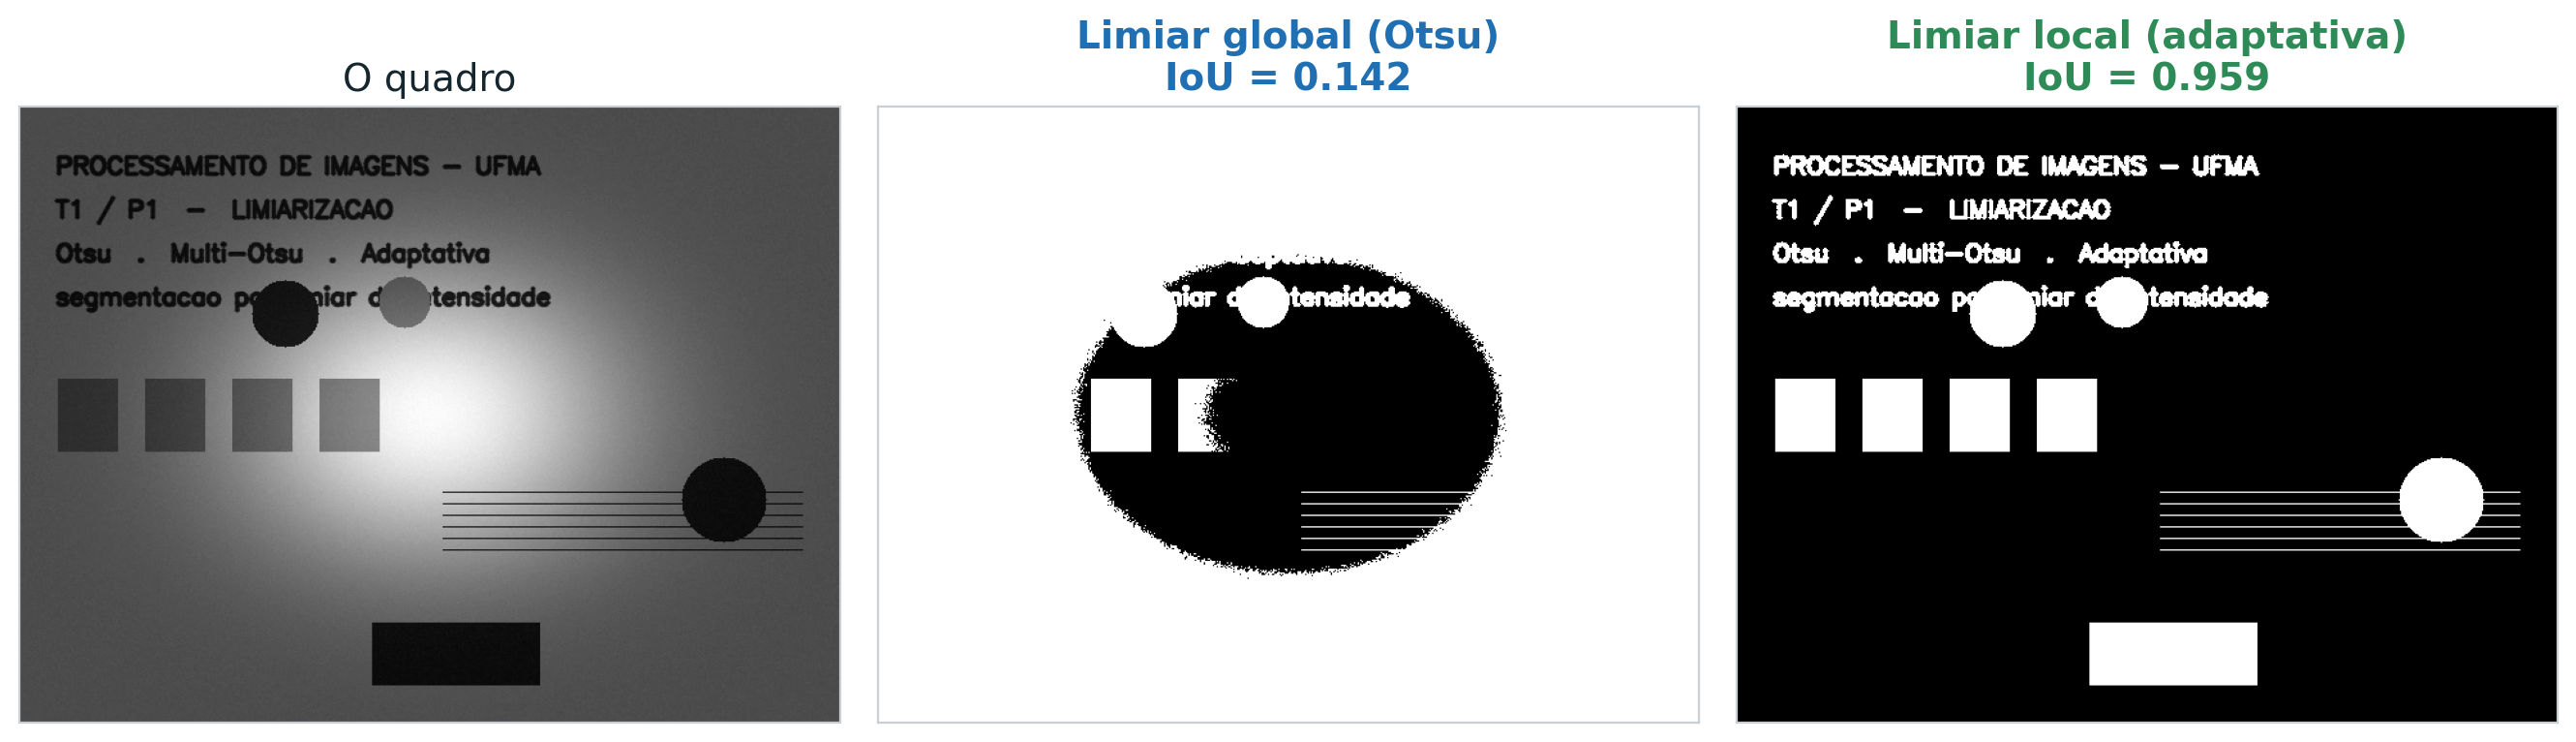
\includegraphics[width=.98\textwidth]{hook_holofote}
  \end{center}

  \vspace{-.3em}
  Mesmo instante, mesmos pixels, mesma cena. \alert{Sete vezes} de diferença.

  \vspace{.4em}
  \sub{A pergunta desta apresentação é por quê — e como saber de antemão qual
  método vai falhar.}

\end{frame}

% =============================================================================
\begin{frame}{Como dividimos}

  \begin{columns}[T,onlytextwidth]
    \column{.33\textwidth}
      \textcolor{cOtsu}{\rule{\textwidth}{2pt}}\\[.4em]
      \otsu{1. Limiar global}\\
      \textbf{Otsu}\\[.5em]
      \sub{\alunoA}\\[.8em]
      \sub{Um limiar para a imagem inteira, escolhido automaticamente.}

    \column{.33\textwidth}
      \textcolor{cMulti}{\rule{\textwidth}{2pt}}\\[.4em]
      \multi{2. Multinível}\\
      \textbf{Multi-Otsu}\\[.5em]
      \sub{\alunoB}\\[.8em]
      \sub{E quando a cena tem três ou mais populações de cinza?}

    \column{.33\textwidth}
      \textcolor{cAdapt}{\rule{\textwidth}{2pt}}\\[.4em]
      \adapt{3. Local}\\
      \textbf{Adaptativa}\\[.5em]
      \sub{\alunoC}\\[.8em]
      \sub{Um limiar diferente para cada pixel.}
  \end{columns}

  \vspace{1.2em}
  Fechamos com a comparação em uma imagem e em um vídeo de 20~s, medindo
  qualidade, estabilidade e custo.

\end{frame}

% =============================================================================
\section{Fundamentos}

% -----------------------------------------------------------------------------
\begin{frame}[fragile]{Limiarização em uma linha}

  Compare cada pixel com um valor de corte $T$ e decida:

  \[
    g(x,y) =
    \begin{cases}
      1 & \text{se } I(x,y) > T \quad \text{(objeto)}\\
      0 & \text{se } I(x,y) \le T \quad \text{(fundo)}
    \end{cases}
  \]

  É a segmentação mais barata que existe: uma comparação por pixel, sem
  treinamento, sem GPU. A saída binária abre caminho para morfologia,
  componentes conexas, OCR.

  \vspace{.6em}
  \begin{fecho}
    Todo o problema se resume a \alert{escolher $T$}. As três técnicas de hoje
    são três respostas diferentes para essa única pergunta.
  \end{fecho}

\end{frame}

% -----------------------------------------------------------------------------
\begin{frame}{De onde vem a dificuldade}

  \begin{center}
    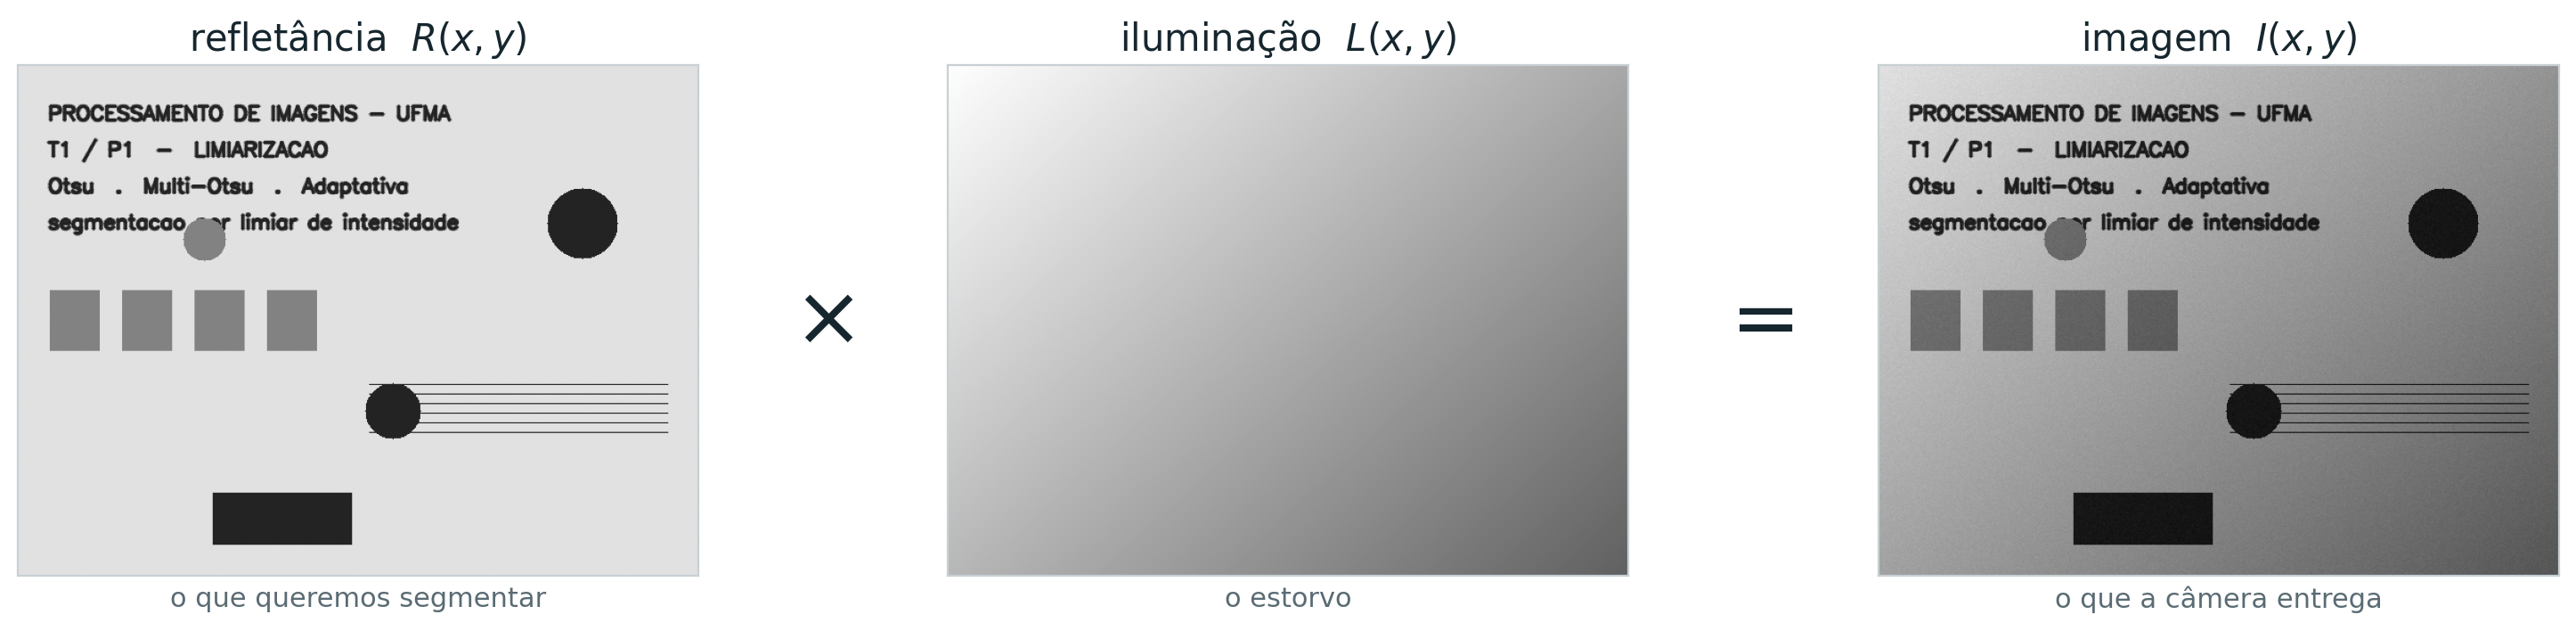
\includegraphics[width=\textwidth]{modelo_formacao}
  \end{center}

  \vspace{-.2em}
  \[
    I(x,y) \;=\; R(x,y)\,\cdot\,L(x,y) \;+\; n(x,y)
  \]

  \vspace{-.3em}
  \sub{A câmera nunca entrega a refletância. Entrega o produto dela pela
  iluminação — e é a refletância que queremos segmentar.}

\end{frame}

% -----------------------------------------------------------------------------
\begin{frame}{A consequência que explica tudo o que vem depois}

  Se $L$ é constante no espaço, comparar $I$ com $T$ equivale a comparar $R$
  com $T/L$. O limiar global é legítimo.

  \vspace{1em}
  \begin{columns}[T,onlytextwidth]
    \column{.48\textwidth}
      \textbf{$L$ muda no \alert{tempo}}\\[.3em]
      \sub{a lâmpada escurece, o obturador muda}\\[.6em]
      O limiar correto apenas \emph{se desloca}. Um método automático
      recalcula e continua funcionando.\\[.5em]
      \textcolor{cAdapt}{\textbf{Não é problema.}}

    \column{.48\textwidth}
      \textbf{$L$ muda no \alert{espaço}}\\[.3em]
      \sub{sombra, holofote, vinheta, dobra do papel}\\[.6em]
      O fundo de uma região escura fica mais escuro que o objeto de uma região
      clara. \emph{Nenhum} $T$ único serve.\\[.5em]
      \textcolor{cMulti}{\textbf{Quebra todo método global.}}
  \end{columns}

  \vspace{1em}
  \sub{Nosso vídeo separa deliberadamente esses dois casos em fases distintas.
  Sem isso, só dá para observar efeitos, não atribuir causas.}

\end{frame}

% -----------------------------------------------------------------------------
\begin{frame}{Como vamos medir}

  \begin{columns}[T,onlytextwidth]
    \column{.52\textwidth}
      \textbf{IoU (Jaccard)} e \textbf{F1 (Dice)}
      \[
        \mathrm{IoU}=\frac{VP}{VP+FP+FN}
        \qquad
        F_1=\frac{2\,VP}{2\,VP+FP+FN}
      \]

      \vspace{.4em}
      \textbf{Instabilidade temporal} — só existe em vídeo:
      \[
        \mathrm{Inst}(k)=\tfrac{1}{N}\bigl|\{\,g_k \neq g_{k-1}\,\}\bigr|
      \]
      \sub{Fração de pixels que trocam de classe entre quadros vizinhos. Como a
      cena quase não muda, valor alto significa cintilação do método.}

    \column{.44\textwidth}
      \begin{block}{Por que não acurácia}
        O objeto ocupa \num{12\,\%} da área.

        \vspace{.5em}
        Um classificador que responde \emph{``tudo é fundo''} acerta
        \num{87,6\,\%} dos pixels.

        \vspace{.5em}
        E tem IoU igual a \num{zero}.
      \end{block}
  \end{columns}

\end{frame}

% -----------------------------------------------------------------------------
\begin{frame}{O material de teste}

  \begin{center}
    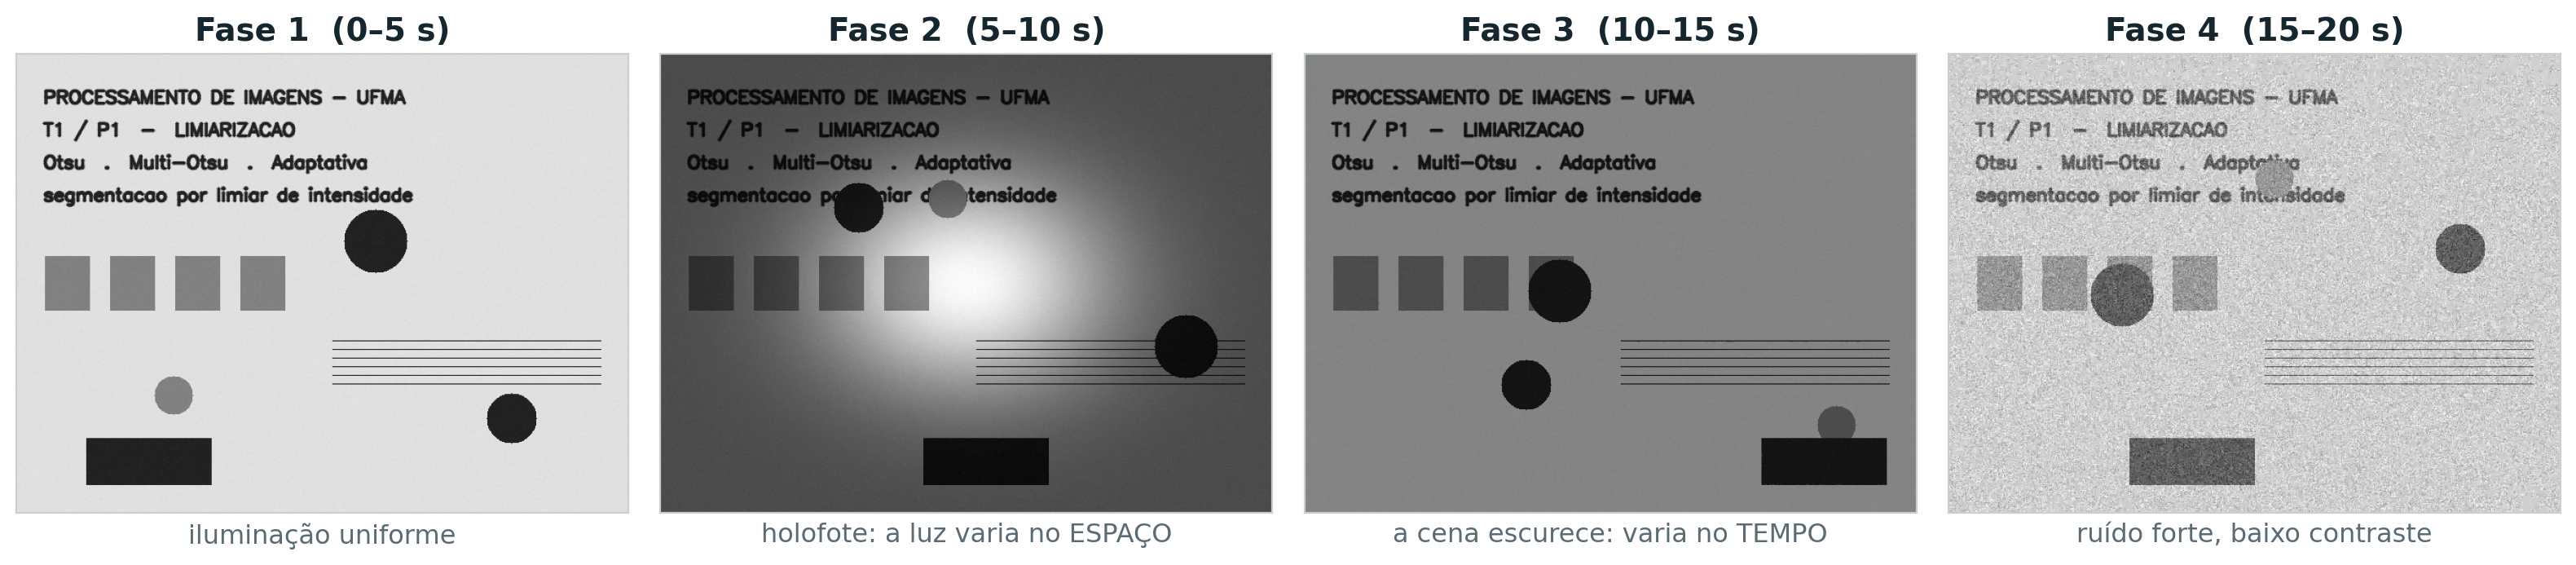
\includegraphics[width=\textwidth]{strip_fases}
  \end{center}

  \vspace{.2em}
  Vídeo de \textbf{20~s}, 640$\times$480, 30~fps — \textbf{600 quadros} — com
  \alert{gabarito analítico quadro a quadro}. Cada fase de 5~s isola um único
  fator de degradação.

  \vspace{.5em}
  \sub{Ter o gabarito exato é o que permite medir IoU por quadro em vez de
  comparar na base do ``parece melhor''. Também usamos três imagens reais do
  acervo do scikit-image (\texttt{camera}, \texttt{coins}, \texttt{page}).}

\end{frame}

% =============================================================================
\section{Otsu: um limiar para a imagem toda}

% -----------------------------------------------------------------------------
\begin{frame}[fragile]{O ponto de partida: o OpenCV pede um número}

  \begin{columns}[T,onlytextwidth]
    \column{.52\textwidth}
      \begin{lstlisting}
T, binaria = cv2.threshold(
    img, 127, 255, cv2.THRESH_BINARY)
      \end{lstlisting}

      \vspace{.3em}
      \footnotesize
      \begin{tabular}{@{}ll@{}}
        \toprule
        \texttt{THRESH\_BINARY}     & $255$ se $src>T$, senão $0$ \\
        \texttt{THRESH\_BINARY\_INV}& $0$ se $src>T$, senão $255$ \\
        \texttt{THRESH\_TRUNC}      & $T$ se $src>T$, senão $src$ \\
        \texttt{THRESH\_TOZERO}     & $src$ se $src>T$, senão $0$ \\
        \texttt{THRESH\_TOZERO\_INV}& $0$ se $src>T$, senão $src$ \\
        \bottomrule
      \end{tabular}

    \column{.44\textwidth}
      \vspace{1.5em}
      Cinco operações diferentes — e todas dependem de um $T$ que \emph{alguém}
      precisa escolher.

      \vspace{.8em}
      Um valor ajustado à mão funciona para uma imagem e falha na seguinte.

      \vspace{.8em}
      \textbf{Otsu (1979) resolve isso lendo o histograma.}
  \end{columns}

\end{frame}

% -----------------------------------------------------------------------------
\begin{frame}{A ideia: agrupar o histograma}

  Trate o histograma normalizado $p(i)=n_i/N$ como uma distribuição de
  probabilidade. Um limiar $t$ a parte em duas classes:

  \vspace{.5em}
  \begin{columns}[T,onlytextwidth]
    \column{.48\textwidth}
      \textbf{Pesos} — quanto cada classe pesa
      \[
        \omega_0(t)=\sum_{i\le t} p(i)
        \qquad
        \omega_1 = 1-\omega_0
      \]
    \column{.48\textwidth}
      \textbf{Médias} — onde cada classe se centra
      \[
        \mu_0(t)=\frac{1}{\omega_0}\sum_{i\le t} i\,p(i)
        \quad
        \mu_1(t)=\frac{\mu_T-\omega_0\mu_0}{\omega_1}
      \]
  \end{columns}

  \vspace{1em}
  \begin{fecho}
    O melhor $t$ é o que deixa as classes \textbf{internamente homogêneas} e
    \textbf{mutuamente distantes}. É agrupamento em uma dimensão, com $k=2$.
  \end{fecho}

\end{frame}

% -----------------------------------------------------------------------------
\begin{frame}{Duas variâncias em disputa}

  \begin{columns}[T,onlytextwidth]
    \column{.48\textwidth}
      \textbf{Dentro} das classes — queremos \alert{pequena}
      \[
        \sigma_W^2(t)=\omega_0\sigma_0^2+\omega_1\sigma_1^2
      \]
      \sub{mede a dispersão interna de cada grupo}

    \column{.48\textwidth}
      \textbf{Entre} as classes — queremos \alert{grande}
      \[
        \sigma_B^2(t)=\omega_0(\mu_0-\mu_T)^2+\omega_1(\mu_1-\mu_T)^2
      \]
      \sub{mede o quanto os grupos se afastam}
  \end{columns}

  \vspace{1.4em}
  Parecem dois objetivos independentes. Não são.

\end{frame}

% -----------------------------------------------------------------------------
\begin{frame}{A identidade que faz o método funcionar}

  \[
    \sigma_T^2 \;=\; \underbrace{\sigma_W^2(t)}_{\text{dentro}}
               \;+\; \underbrace{\sigma_B^2(t)}_{\text{entre}}
    \qquad\text{para \emph{todo} } t
  \]

  \pause
  \vspace{.2em}
  \sub{Esboço: separe $\sigma_T^2$ nas duas classes e escreva
  $i-\mu_T=(i-\mu_0)+(\mu_0-\mu_T)$ dentro de $C_0$. O termo cruzado some,
  porque $\sum_{C_0}(i-\mu_0)p(i)=0$ por definição de $\mu_0$.}

  \pause
  \vspace{.4em}
  $\sigma_T^2$ depende só da imagem, \textbf{não de $t$}. Logo:

  \[
    \text{maximizar } \sigma_B^2(t)
    \;\;\equiv\;\;
    \text{minimizar } \sigma_W^2(t)
  \]

  \pause
  \vspace{-.4em}
  \begin{fecho}
    E $\sigma_B^2$ só precisa de \textbf{médias} — por isso é ele que se maximiza.
  \end{fecho}

\end{frame}

% -----------------------------------------------------------------------------
\begin{frame}{O critério, e ele em ação}

  \vspace{-.2em}
  \begin{center}
    $\displaystyle \sigma_B^2(t)=\omega_0\,\omega_1\,(\mu_0-\mu_1)^2$
    \qquad\qquad
    $\displaystyle t^{*}=\arg\max_t \;\sigma_B^2(t)$
  \end{center}

  \vspace{-.1em}
  \begin{center}
    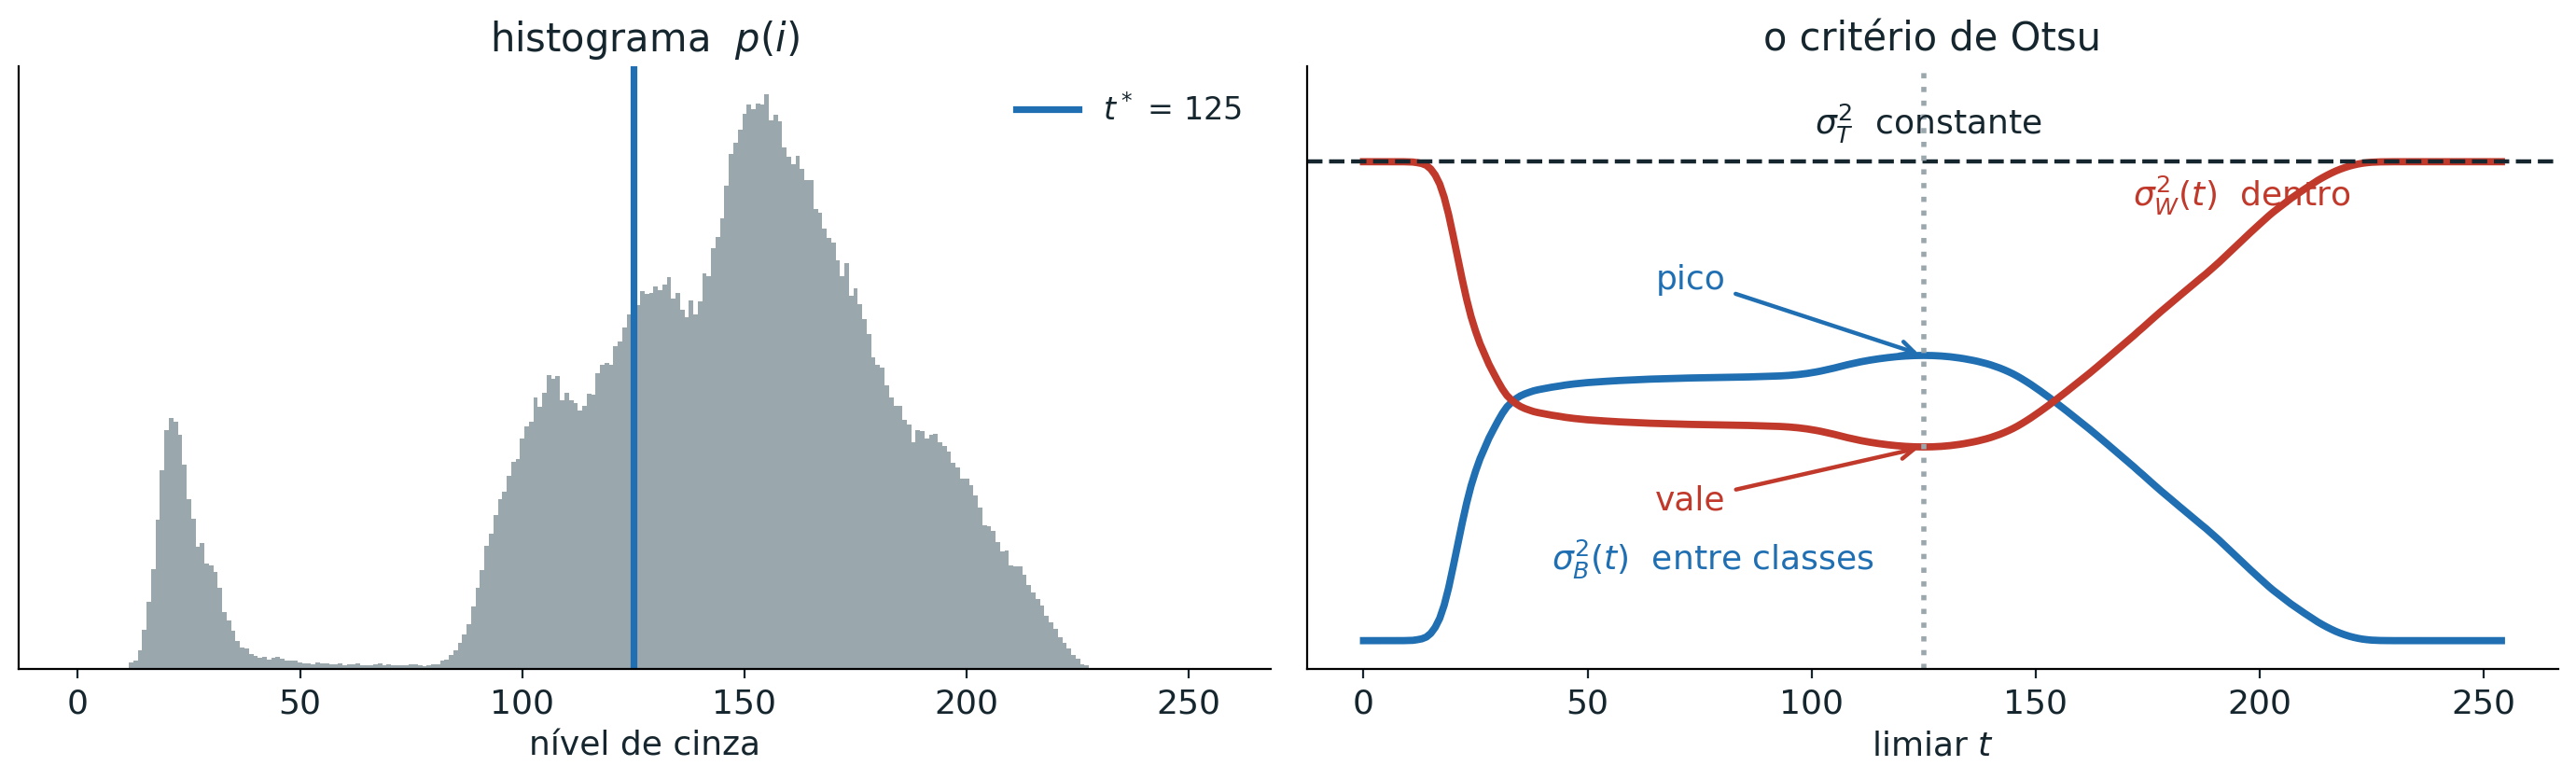
\includegraphics[width=\textwidth]{otsu_anatomia}
  \end{center}

  \vspace{-.5em}
  \sub{$\omega_0\omega_1$ premia classes de tamanhos parecidos,
  $(\mu_0-\mu_1)^2$ premia classes bem separadas. O pico de uma curva cai
  exatamente no vale da outra.}

\end{frame}

% -----------------------------------------------------------------------------
\begin{frame}{Custo e autodiagnóstico}

  \begin{columns}[T,onlytextwidth]
    \column{.48\textwidth}
      \textbf{Uma única passada pela imagem}

      \vspace{.5em}
      Com somas acumuladas obtemos $\omega_0(t)$ e $\mu(t)$ para todos os $t$ de
      uma vez:
      \[
        O(N+L)\;\approx\;O(N)
      \]

      \vspace{.4em}
      Medido: \num{0,16~ms} por quadro de 640$\times$480 no OpenCV.
      Cerca de \num{6\,400} quadros por segundo.

    \column{.48\textwidth}
      \textbf{Separabilidade $\eta$}
      \[
        \eta=\frac{\sigma_B^2(t^{*})}{\sigma_T^2}\in[0,1]
      \]

      \vspace{.3em}
      \footnotesize
      \begin{tabular}{@{}lcc@{}}
        \toprule
        Imagem & $t^{*}$ & $\eta$ \\
        \midrule
        \texttt{camera}    & 102 & \textbf{0,857} \\
        \texttt{coins}     & 107 & 0,756 \\
        \texttt{page}      & 157 & 0,719 \\
        sintética (luz desigual) & 125 & \textbf{0,596} \\
        \bottomrule
      \end{tabular}

      \vspace{.6em}
      \sub{$\eta$ baixo avisa que o histograma não é bimodal — ou seja, que o
      limiar global vai decepcionar.}
  \end{columns}

\end{frame}

% -----------------------------------------------------------------------------
\begin{frame}{Otsu não está sozinho}

  \vspace{-.4em}
  \begin{center}
    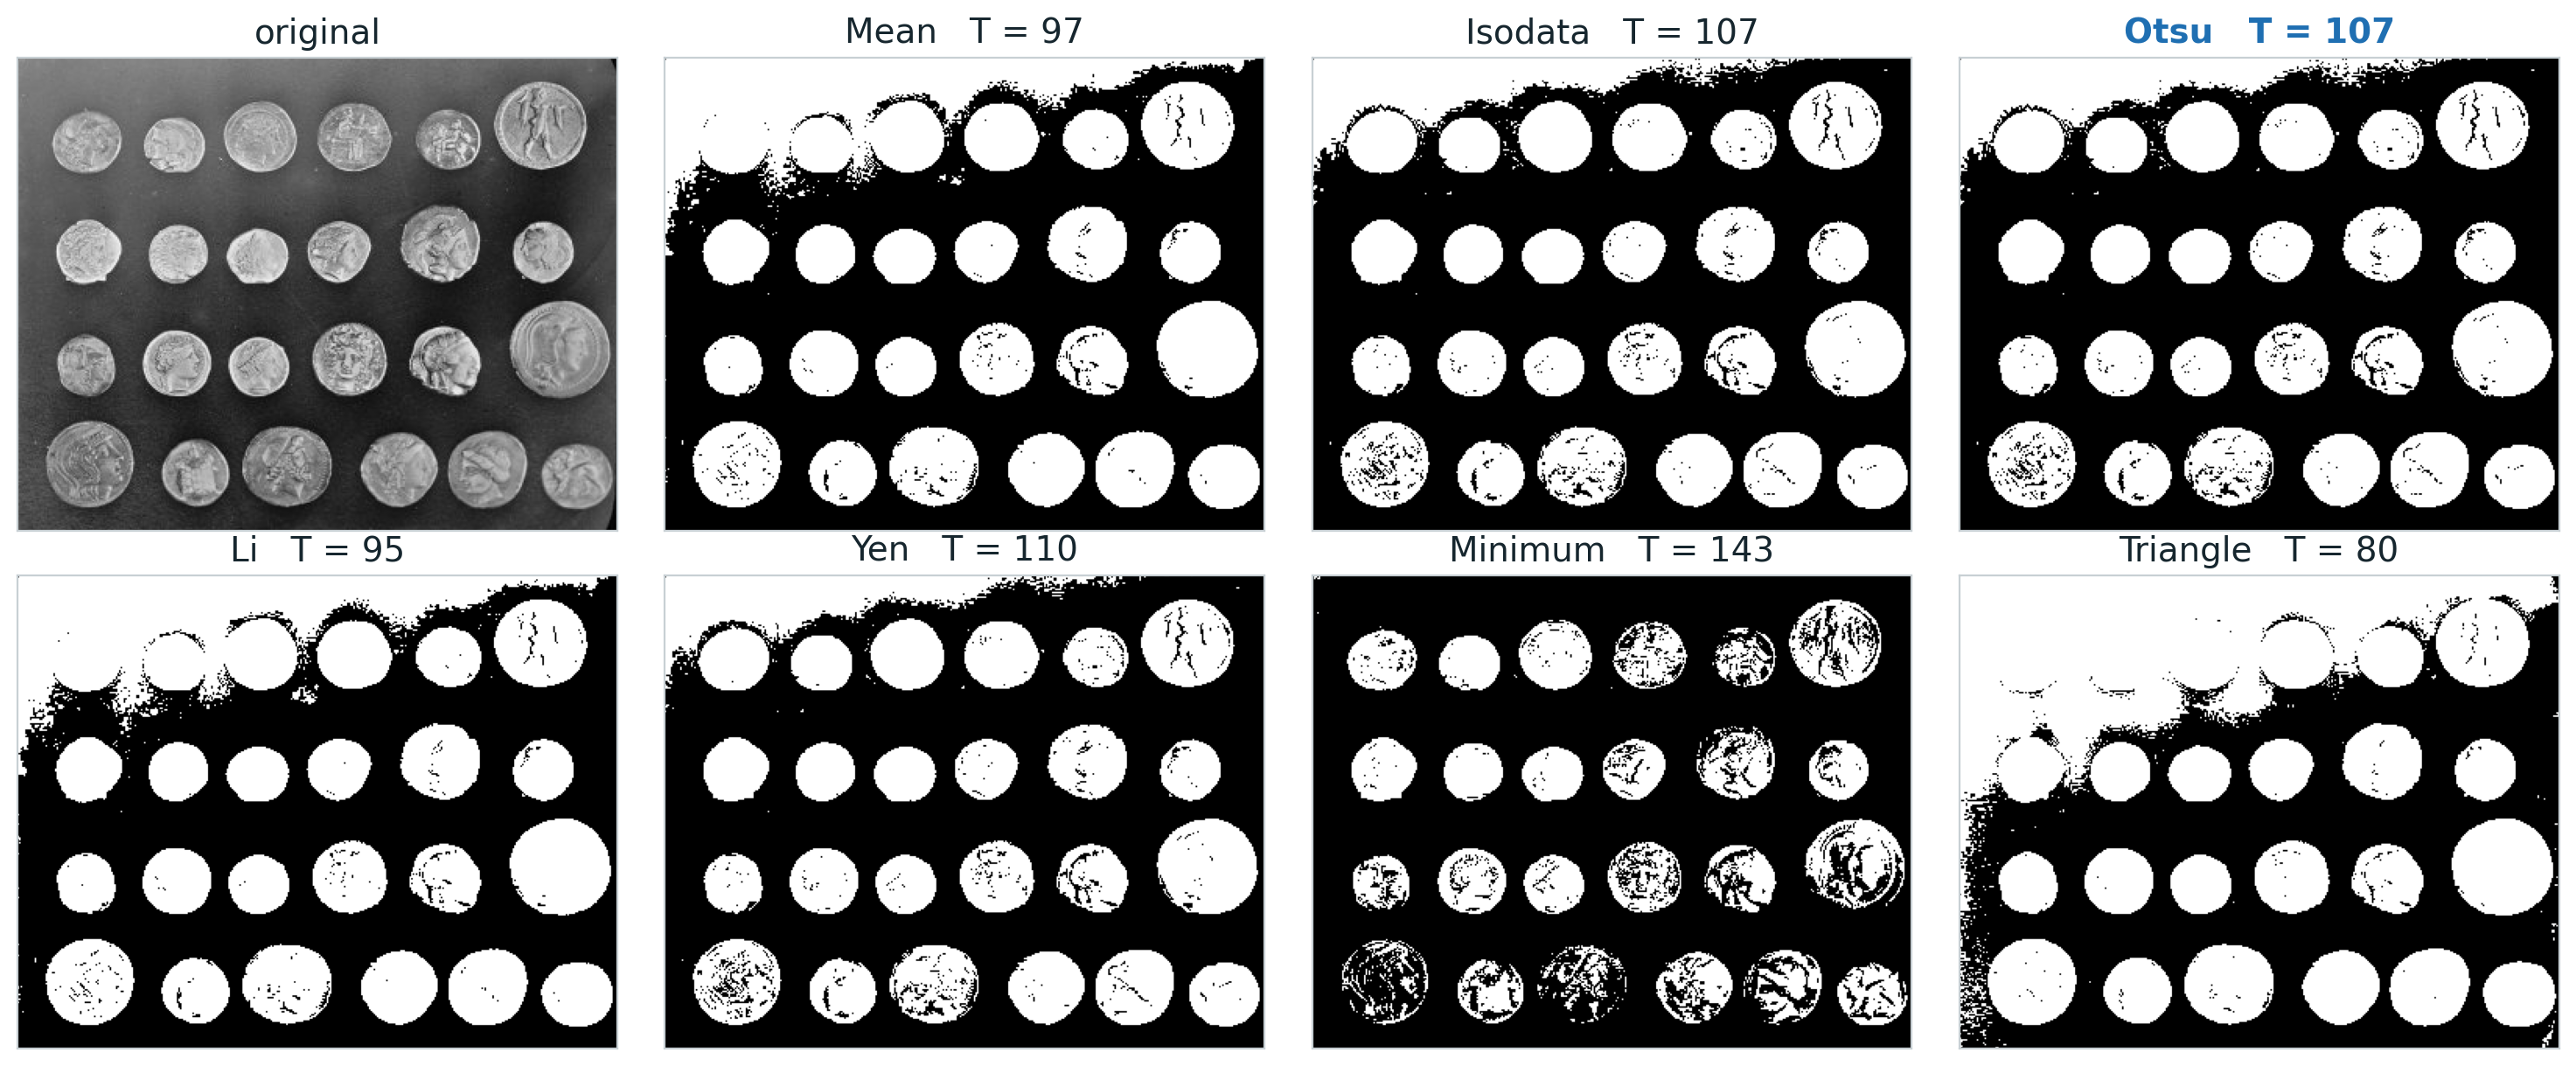
\includegraphics[width=.80\textwidth]{try_all_paisagem}
  \end{center}

  \vspace{-.5em}
  \begin{columns}[T,onlytextwidth]
    \column{.50\textwidth}
      \scriptsize
      \begin{tabular}{@{}ll@{}}
        Mean      & $T=\mu_T$ \\
        Isodata   & ponto fixo de $T=\tfrac{\mu_0+\mu_1}{2}$ \\
        \textbf{Otsu} & $\max \sigma_B^2$ \\
        Li        & mínima entropia cruzada \\
      \end{tabular}
    \column{.50\textwidth}
      \scriptsize
      \begin{tabular}{@{}ll@{}}
        Yen       & máxima correlação entrópica \\
        Minimum   & vale entre os dois modos suavizados \\
        Triangle  & máx.\ distância à reta pico--extremo \\
        & \\
      \end{tabular}
  \end{columns}

  \vspace{.1em}
  \sub{Quase todos coincidem quando o histograma é bimodal. Divergem se o objeto
  é pequeno, ou se o histograma é unimodal — o caso do Triangle.}

\end{frame}

% -----------------------------------------------------------------------------
\begin{frame}{O que o Otsu entrega — e o que não entrega}

  \begin{columns}[T,onlytextwidth]
    \column{.48\textwidth}
      \textbf{Fase 3} — a cena escurece por completo

      \vspace{.5em}
      O limiar desce sozinho de \num{147} para \num{47}.

      \vspace{.5em}
      IoU: \textbf{0,944} $\rightarrow$ \textbf{0,947}.

      \vspace{.5em}
      \textcolor{cAdapt}{Praticamente invariante a mudança \textbf{global} de
      luz.}

    \column{.48\textwidth}
      \textbf{Fase 2} — a luz varia dentro do quadro

      \vspace{.5em}
      O limiar continua ``ótimo''. Só que ótimo não basta.

      \vspace{.5em}
      IoU: \textbf{0,944} $\rightarrow$ \textcolor{cMulti}{\textbf{0,139}}.

      \vspace{.5em}
      \textcolor{cMulti}{Colapso total com variação \textbf{espacial}.}
  \end{columns}

  \vspace{1.2em}
  \begin{fecho}
    Dizer que ``Otsu falha com iluminação variável'' é \alert{impreciso}.
    Ele falha com variação \textbf{espacial} de iluminação.
  \end{fecho}

\end{frame}

% =============================================================================
\section{Multi-Otsu: e se houver três populações?}

% -----------------------------------------------------------------------------
\begin{frame}{Duas classes raramente bastam}

  \begin{columns}[T,onlytextwidth]
    \column{.42\textwidth}
      \footnotesize
      \begin{tabular}{@{}ll@{}}
        \toprule
        \textbf{Cena} & \textbf{Populações} \\
        \midrule
        Documento  & papel, tinta, \textbf{sombra} \\
        Radiografia& fundo, tecido, \textbf{osso} \\
        Satélite   & água, vegetação, \textbf{solo} \\
        Esteira    & esteira, peça, \textbf{sombra} \\
        \bottomrule
      \end{tabular}

      \vspace{1em}
      \normalsize
      Forçar duas classes onde há três significa \alert{fundir} duas
      populações distintas. A informação perdida não volta.

    \column{.54\textwidth}
      \[
        \sigma_B^2 = \sum_{k=0}^{M-1}\omega_k(\mu_k-\mu_T)^2
      \]
      \[
        (t_1^{*},\dots,t_{M-1}^{*})=\arg\max \;\sigma_B^2
      \]

      \vspace{.5em}
      \sub{Mesmo critério do Otsu, agora com $M$ classes e $M-1$ limiares.
      A identidade $\sigma_T^2=\sigma_W^2+\sigma_B^2$ continua valendo —
      a demonstração se repete classe a classe.}
  \end{columns}

\end{frame}

% -----------------------------------------------------------------------------
\begin{frame}{O problema: a busca explode}

  \begin{columns}[c,onlytextwidth]
    \column{.46\textwidth}
      \footnotesize
      \begin{tabular}{@{}cccl@{}}
        \toprule
        $M$ & limiares & combinações & \\
        \midrule
        2 & 1 & 255 & trivial \\
        3 & 2 & 32\,385 & tranquilo \\
        4 & 3 & 2\,731\,135 & minutos \\
        5 & 4 & \textbf{172\,061\,505} & \textcolor{cMulti}{inviável} \\
        6 & 5 & $8{,}6\times10^{9}$ & impossível \\
        \bottomrule
      \end{tabular}

      \vspace{.8em}
      \normalsize
      $\displaystyle \binom{L-1}{M-1}$ combinações, cada uma com $O(L)$
      operações.

    \column{.50\textwidth}
      \begin{block}{Aconteceu com a gente}
        A primeira versão do nosso código usava
        \texttt{itertools.combinations}.

        \vspace{.5em}
        $M=3$: milissegundos. \\
        $M=4$: minutos. \\
        $M=5$: \alert{travou}.

        \vspace{.5em}
        \sub{Foi o que nos obrigou a procurar a formulação correta.}
      \end{block}
  \end{columns}

\end{frame}

% -----------------------------------------------------------------------------
\begin{frame}{A saída: tabelas de momentos + programação dinâmica}

  \textbf{1. Pré-compute os momentos de todo intervalo} \sub{(Liao, Chen \& Chung, 2001)}
  \[
    P(u,v)=\sum_{i=u}^{v}p(i)
    \qquad
    S(u,v)=\sum_{i=u}^{v}i\,p(i)
    \qquad
    H(u,v)=\frac{S(u,v)^2}{P(u,v)}
  \]

  \vspace{-.2em}
  \sub{Vale $\sigma_B^2=\sum_k H(u_k,v_k)-\mu_T^2$; como $\mu_T^2$ é constante,
  basta maximizar $J=\sum_k H$. Cada avaliação cai de $O(L)$ para $O(M)$.}

  \vspace{.6em}
  \textbf{2. Explore que $J$ é aditiva em intervalos contíguos}
  \[
    D[1][v]=H(0,v)
    \qquad
    D[m][v]=\max_{u<v}\Bigl(D[m-1][u]+H(u{+}1,v)\Bigr)
  \]

  \vspace{-.1em}
  \begin{fecho}
    $O\!\left(\binom{L}{M-1}M\right) \;\longrightarrow\; \mathbf{O(M L^2)}$.
    \enspace Para $M=5$: de $1{,}7\times10^{8}$ avaliações para
    $3{,}3\times10^{5}$ operações — de \emph{horas} para \num{1,5~ms}.
  \end{fecho}

\end{frame}

% -----------------------------------------------------------------------------
\begin{frame}{Quantas classes usar?}

  \begin{columns}[T,onlytextwidth]
    \column{.60\textwidth}
      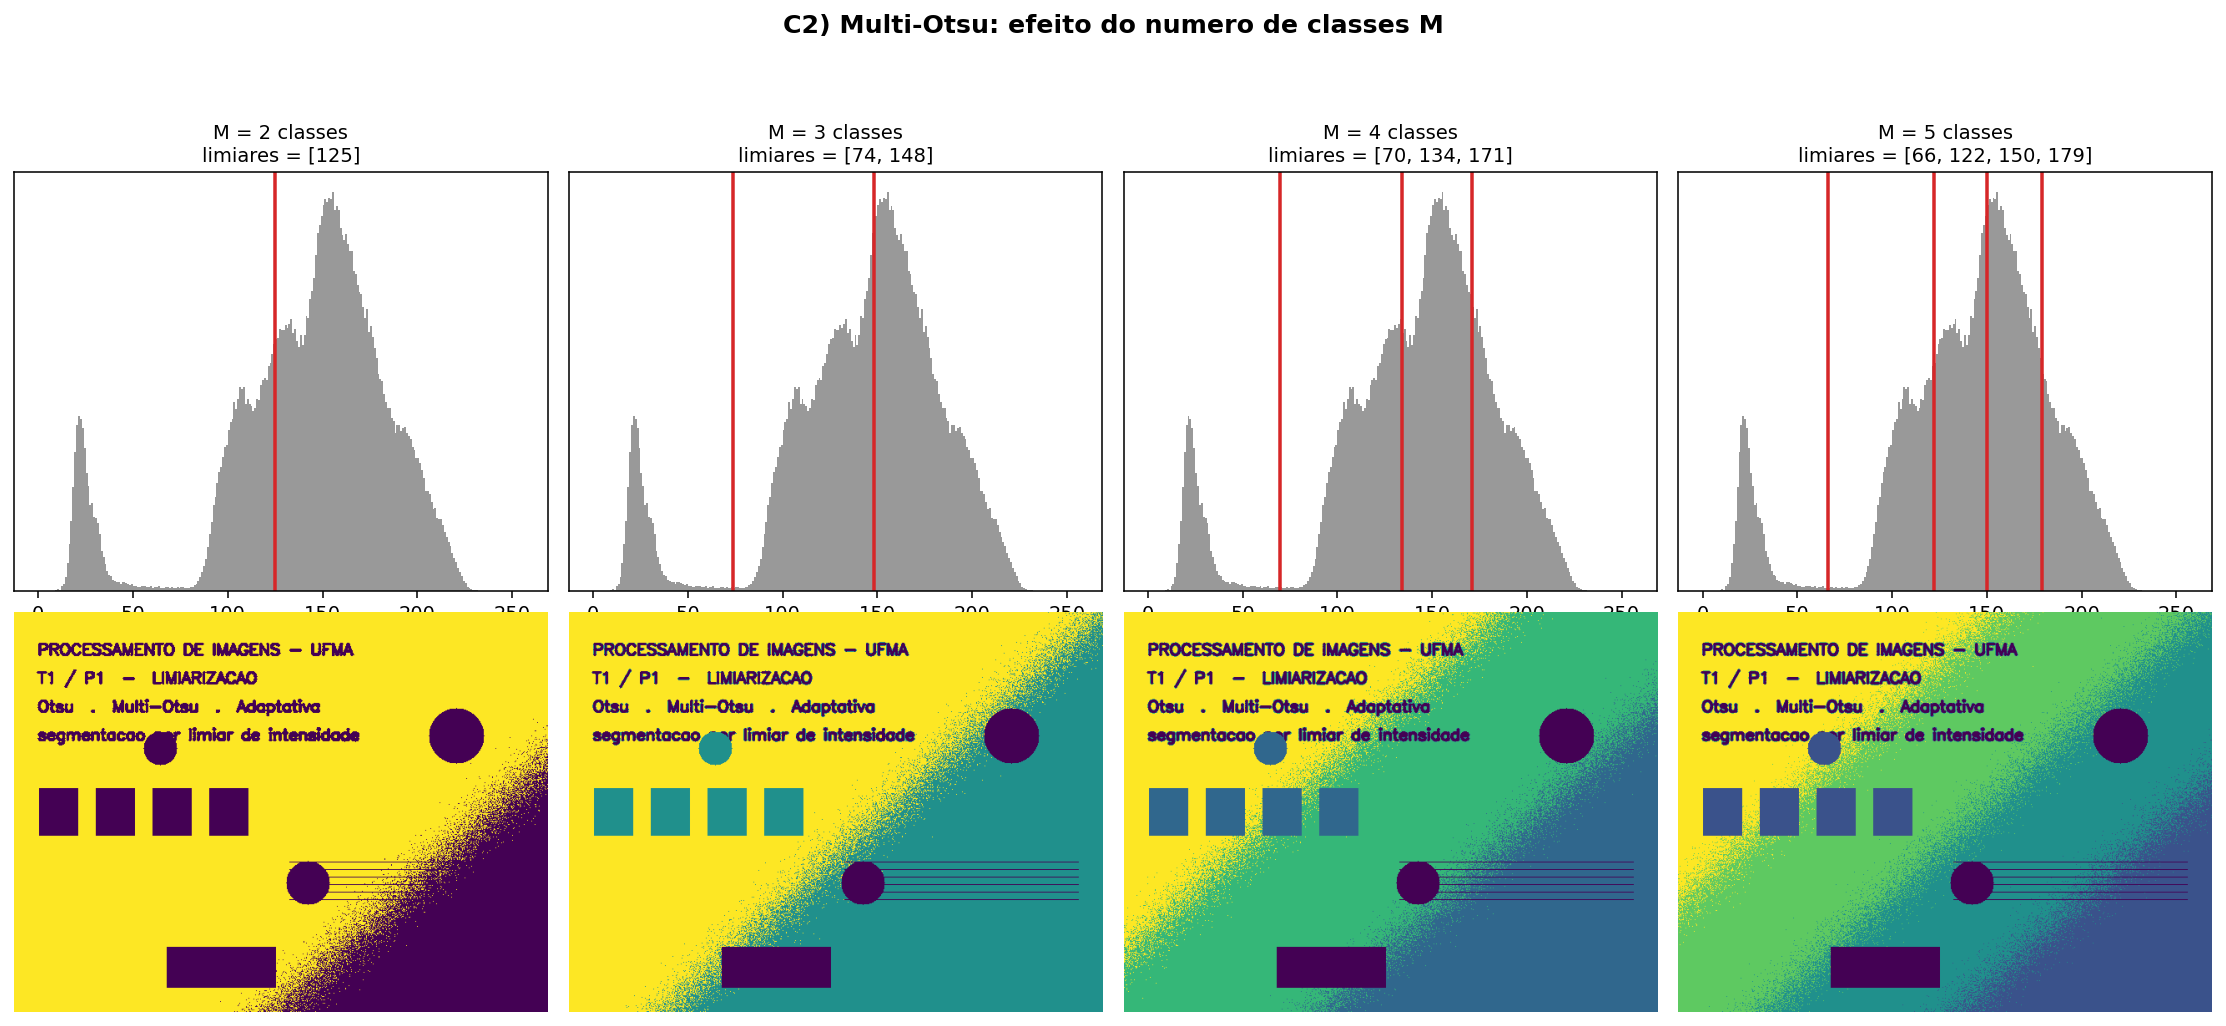
\includegraphics[width=\textwidth]{C2_multiotsu_M_04_sintetica}
    \column{.36\textwidth}
      \vspace{.5em}
      Aumentar $M$ \textbf{sempre} aumenta $\sigma_B^2$ — no limite $M=L$ e
      $\sigma_B^2=\sigma_T^2$.

      \vspace{.7em}
      \alert{Logo $M$ não se escolhe maximizando $\sigma_B^2$} — seria como
      escolher o número de parâmetros de um modelo pelo ajuste.

      \vspace{.7em}
      Vale conhecimento do domínio, o cotovelo da curva, ou AIC/BIC.
      $M$ é hiperparâmetro, não resultado.
  \end{columns}

\end{frame}

% -----------------------------------------------------------------------------
\begin{frame}{O achado: qual limiar você usa muda tudo}

  Com 3 classes saem dois limiares. Para obter uma máscara binária é preciso
  decidir onde cortar — e essa decisão é do projetista.

  \vspace{.8em}
  \begin{columns}[T,onlytextwidth]
    \column{.48\textwidth}
      \multi{Corte em $t_2$} \sub{(escura + média)}

      \vspace{.4em}
      Fase 1: IoU \textbf{0,966} — o \emph{melhor método global} do trabalho.

      \vspace{.4em}
      Fase 2 (holofote): \textcolor{cMulti}{\textbf{0,138}}.

    \column{.48\textwidth}
      \multi{Corte em $t_1$} \sub{(só a classe mais escura)}

      \vspace{.4em}
      Fase 1: IoU 0,592 — perde os objetos de cinza médio.

      \vspace{.4em}
      Fase 2 (holofote): \textcolor{cAdapt}{\textbf{0,731}}.
  \end{columns}

  \vspace{.8em}
  \sub{O holofote rebaixa o fundo até $\approx 76$ — \emph{acima} de
  $t_1\approx52$, muito \emph{abaixo} de $t_2\approx131$. A classe mais escura
  tem uma margem de segurança que as outras não têm.}

  \vspace{.4em}
  \begin{fecho}
    Mesmo método, mesmo quadro, mesmo histograma: \alert{5,3$\times$} de
    diferença só na escolha do corte.
  \end{fecho}

\end{frame}

% =============================================================================
\section{Adaptativa: um limiar por pixel}

% -----------------------------------------------------------------------------
\begin{frame}{Abandonar o limiar único}

  \begin{center}
    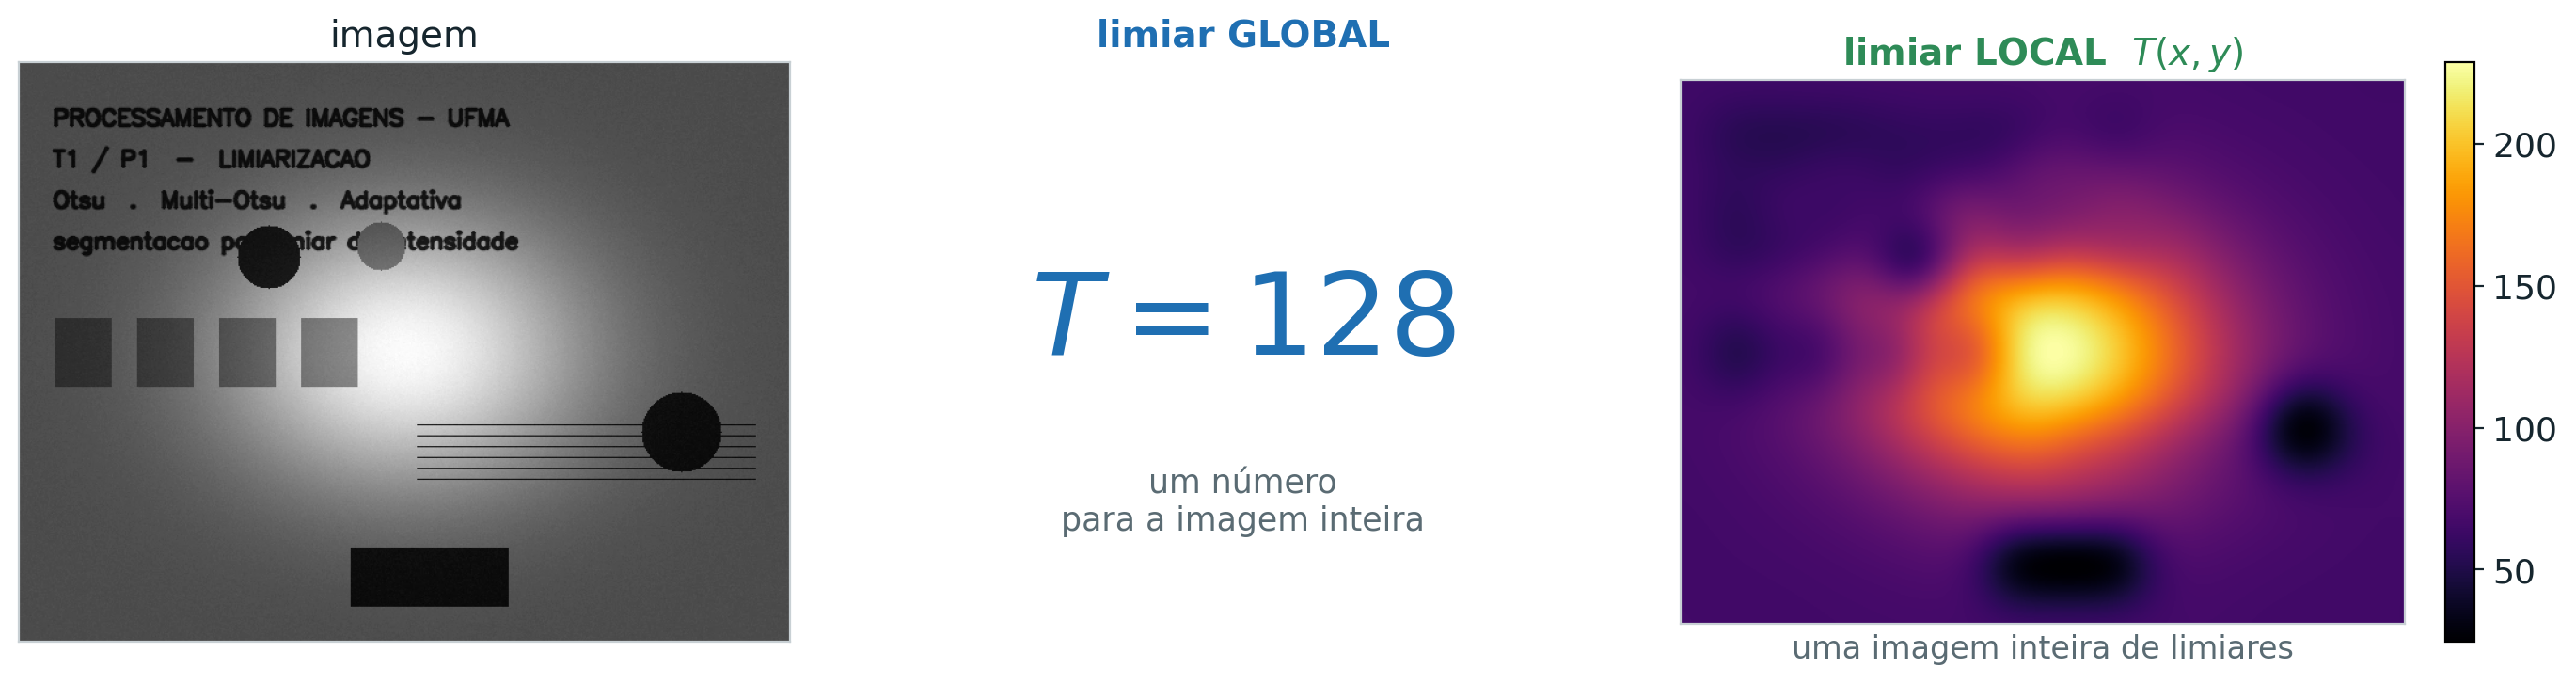
\includegraphics[width=.95\textwidth]{limiar_global_vs_local}
  \end{center}

  \vspace{-.2em}
  Como $L(x,y)$ varia devagar no espaço, dentro de uma janela pequena ela é
  quase constante — e ali um limiar local é válido.

  \vspace{.4em}
  \sub{Em linguagem de frequências: $\log I=\log R+\log L$, e a iluminação é a
  componente de baixa frequência. A limiarização adaptativa é um passa-altas
  seguido de um limiar fixo.}

\end{frame}

% -----------------------------------------------------------------------------
\begin{frame}[fragile]{As duas fórmulas, e o papel de $C$}

  \begin{columns}[T,onlytextwidth]
    \column{.52\textwidth}
      \begin{lstlisting}
cv2.adaptiveThreshold(src, 255,
    cv2.ADAPTIVE_THRESH_GAUSSIAN_C,
    cv2.THRESH_BINARY, blockSize, C)
      \end{lstlisting}

      \vspace{.2em}
      \textbf{Média:} $\;T(x,y)=\dfrac{1}{b^2}\displaystyle\sum_{B_b(x,y)} I - C$

      \vspace{.3em}
      \textbf{Gaussiana:} $\;T(x,y)=\displaystyle\sum_{B_b(x,y)} w\,I - C$

      \vspace{.8em}
      \sub{Atenção: com \texttt{blockSize=35} a gaussiana usa
      $\sigma=5{,}6$, ou seja, enxerga uns $\pm 11$~px — bem menos que os 35
      nominais.}

    \column{.44\textwidth}
      \begin{block}{Sem $C$, só ruído}
        Em região homogênea $I\approx m$, e o teste $I>m$ vira o
        \alert{sinal do ruído}.

        \vspace{.4em}
        $C$ cria uma banda morta: só é objeto quem for pelo menos $C$ níveis
        mais escuro que a vizinhança.
        \[
          \text{objeto} \iff m(x,y)-I(x,y)>C
        \]
      \end{block}
  \end{columns}

\end{frame}

% -----------------------------------------------------------------------------
\begin{frame}{Por que isso roda em tempo real}

  A média em janela $b\times b$ custaria $O(N b^2)$ — para $b=151$ seriam umas
  23\,000 somas \emph{por pixel}. A \textbf{imagem integral} resolve com quatro
  acessos:

  \[
    II(x,y)=\sum_{x'\le x}\sum_{y'\le y} I(x',y')
  \]
  \[
    \textstyle\sum_{\text{retângulo}} I
    = II(x_2,y_2)-II(x_1{-}1,y_2)-II(x_2,y_1{-}1)+II(x_1{-}1,y_1{-}1)
  \]

  \vspace{.6em}
  \footnotesize
  \begin{tabular}{@{}lcc@{}}
    \toprule
     & Custo total & Depende de $b$? \\
    \midrule
    Soma direta & $O(Nb^2)$ & sim, quadraticamente \\
    \textbf{Imagem integral} & $\mathbf{O(N)}$ & \textbf{não} \\
    \bottomrule
  \end{tabular}

  \vspace{.5em}
  \normalsize
  \sub{Crow (1984), aplicado à limiarização por Bradley \& Roth (2007).}

\end{frame}

% -----------------------------------------------------------------------------
\begin{frame}{A regra prática que quase nos enganou}

  \begin{center}
    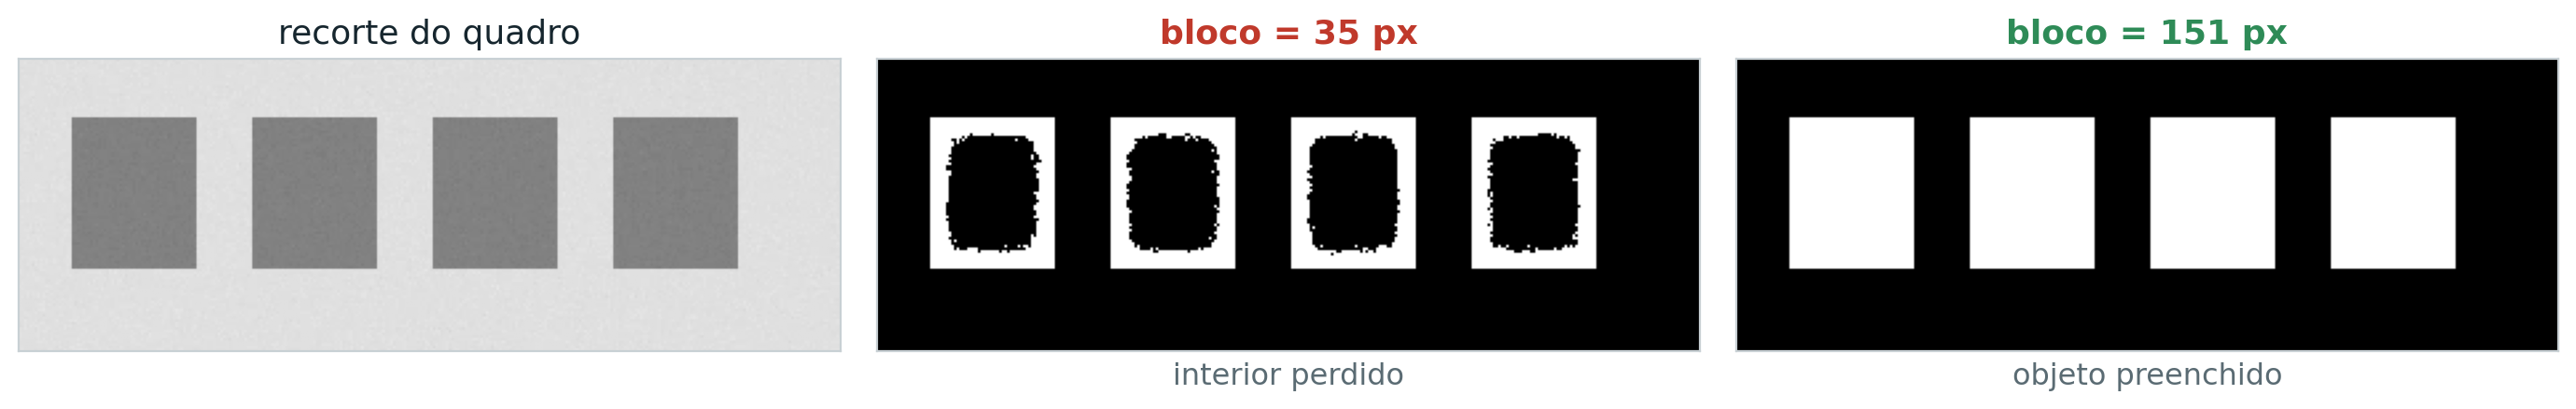
\includegraphics[width=.95\textwidth]{esvaziamento}
  \end{center}

  \vspace{.2em}
  Um pixel no centro de um objeto grande tem a vizinhança \emph{inteira} dentro
  do objeto. Logo $m\approx I$, o teste falha, e só a borda sobrevive.

  \vspace{.6em}
  \[
    \underbrace{\text{maior objeto}}_{130\text{ px}}
    \;<\; b \;<\;
    \underbrace{\text{escala de variação da luz}}_{300\text{ px}}
  \]

\end{frame}

% -----------------------------------------------------------------------------
\begin{frame}{O efeito medido}

  \footnotesize
  \begin{center}
  \begin{tabular}{@{}lccccccc@{}}
    \toprule
    \textbf{bloco} & 35 & 71 & 101 & 131 & \textbf{151} & 201 & 301 \\
    \midrule
    Fase 1 & 0,627 & 0,876 & 0,964 & 0,968 & \textbf{0,971} & 0,975 & 0,980 \\
    Fase 2 & 0,532 & 0,761 & 0,914 & 0,957 & \textbf{0,959} & 0,963 & 0,969 \\
    Fase 3 & 0,570 & 0,784 & 0,926 & 0,941 & \textbf{0,946} & 0,955 & 0,970 \\
    Fase 4 & 0,240 & 0,309 & 0,354 & 0,386 & \textbf{0,401} & 0,425 & 0,451 \\
    \bottomrule
  \end{tabular}
  \end{center}

  \vspace{1em}
  \normalsize
  Com o valor ``de livro-texto'' $b=35$, a adaptativa parecia \emph{pior que o
  Otsu global}. Com $b=151$, o IoU médio no vídeo vai de
  \num{0,513} para \num{0,863}.

  \vspace{.8em}
  \begin{fecho}
    Um método pode parecer inferior só porque seus hiperparâmetros não foram
    ajustados à \alert{escala do problema}. Mantivemos as duas configurações
    lado a lado nos resultados.
  \end{fecho}

\end{frame}

% -----------------------------------------------------------------------------
\begin{frame}{Sauvola: deixar o desvio local escolher o $C$}

  \[
    T(x,y)=m(x,y)\left[\,1+k\left(\frac{s(x,y)}{R}-1\right)\right]
    \qquad R=128,\;\; k\approx0{,}2
  \]

  \vspace{.6em}
  \begin{columns}[T,onlytextwidth]
    \column{.48\textwidth}
      \textbf{Região homogênea} $s\to0$
      \[ T \to m\,(1-k) \]
      O limiar desce sozinho abaixo da média local — a banda morta aparece
      \emph{automaticamente}.

    \column{.48\textwidth}
      \textbf{Região de alto contraste} $s\to R$
      \[ T \to m \]
      A sensibilidade volta.
  \end{columns}

  \vspace{.8em}
  No vídeo: instabilidade temporal de \adapt{1,58\,\%} contra \num{6,00\,\%} da
  adaptativa do OpenCV — e, na fase de ruído, \adapt{4,34\,\%} contra
  \num{21,95\,\%}.

\end{frame}

% =============================================================================
\section{Comparação}

% -----------------------------------------------------------------------------
\begin{frame}{O limiar em movimento}

  \vspace{-.3em}
  \begin{center}
    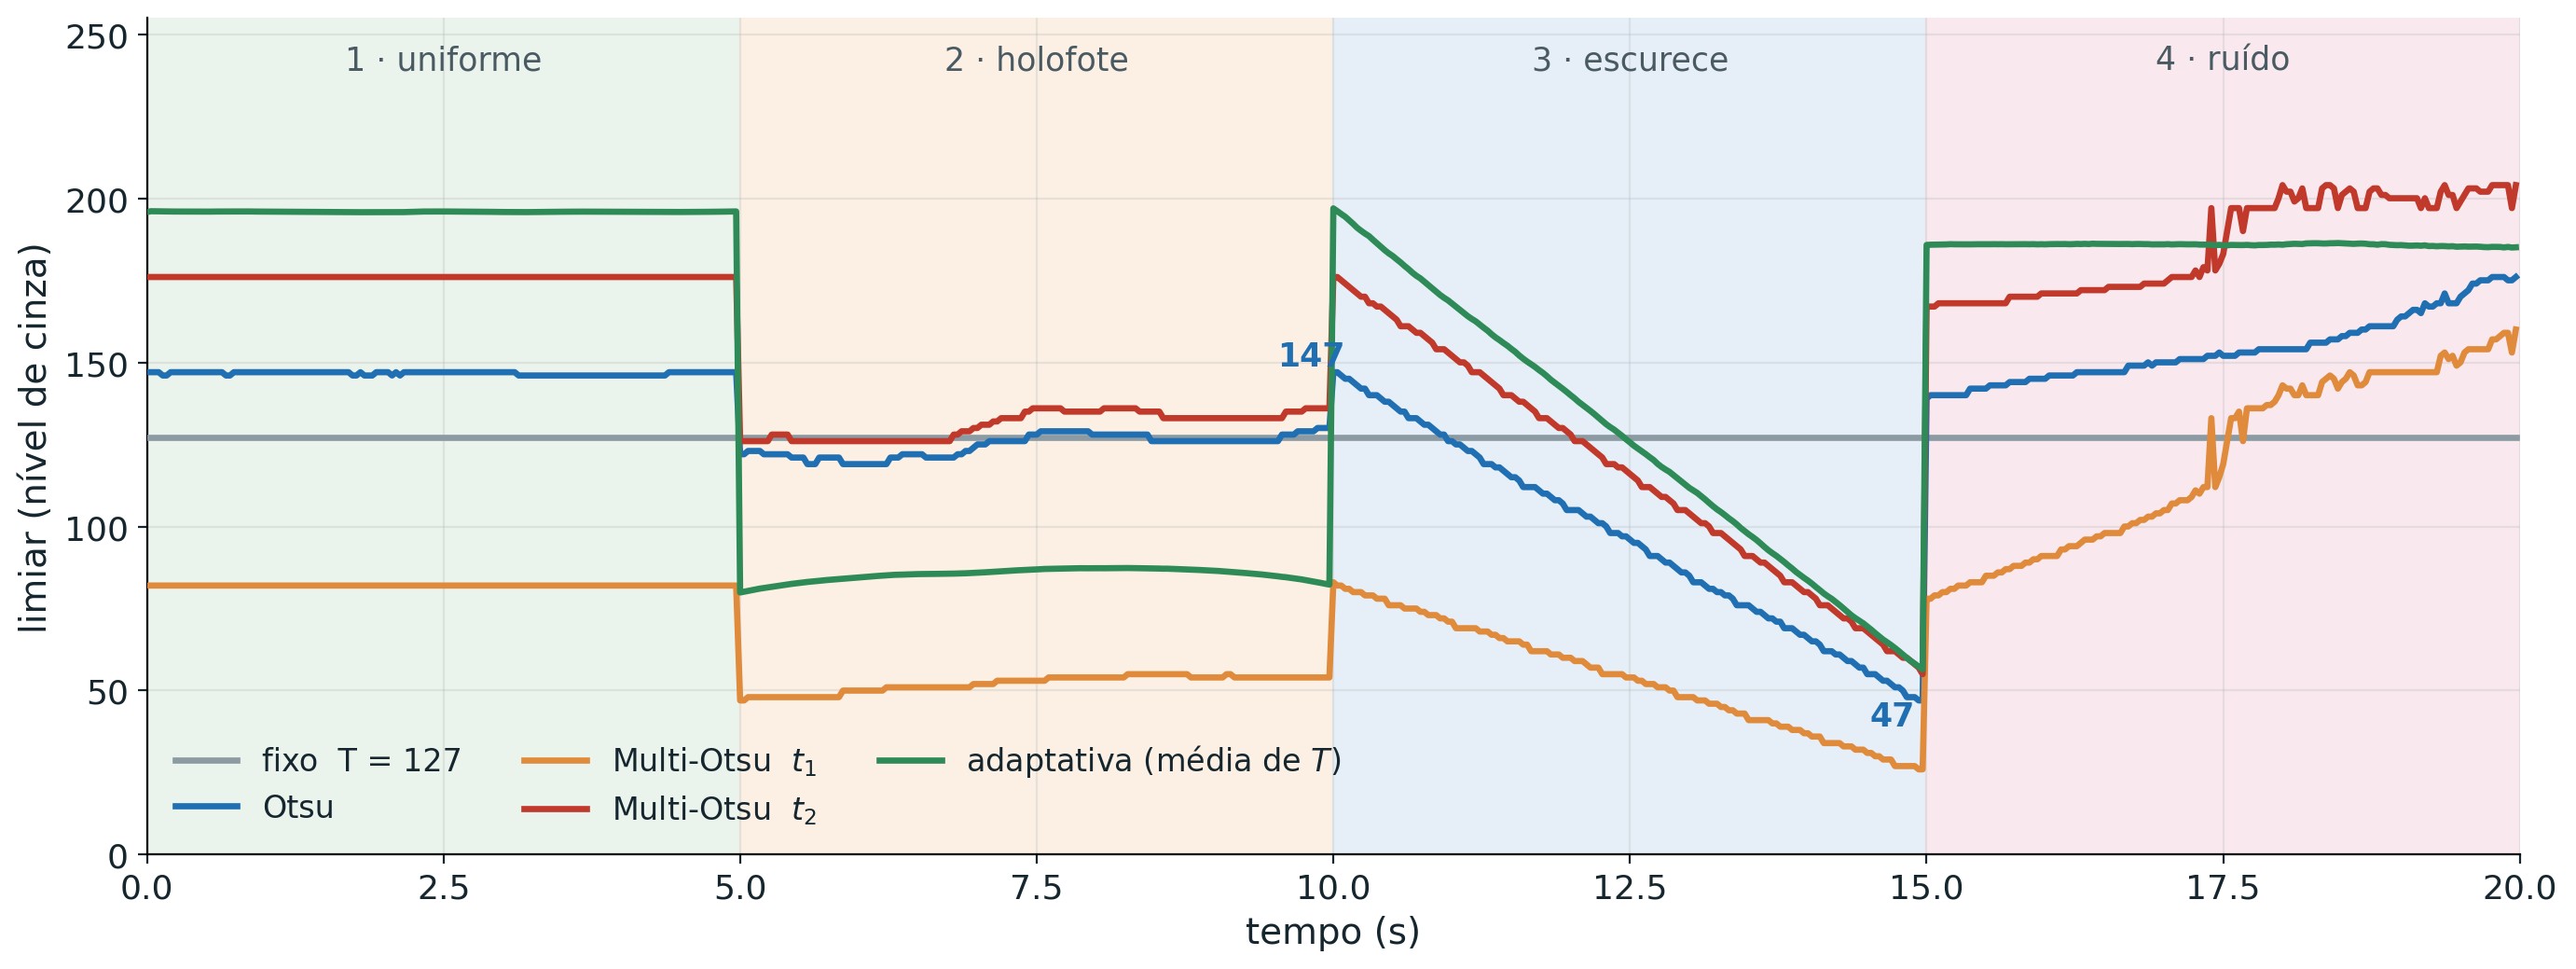
\includegraphics[width=.94\textwidth]{limiar_no_tempo_slide}
  \end{center}

  \vspace{-.5em}
  \sub{Fase 3: enquanto a cena escurece, o limiar do Otsu desce de 147 para 47 —
  e o IoU não se mexe. O limiar fixo, em cinza, segue reto em 127.}

\end{frame}

% -----------------------------------------------------------------------------
\begin{frame}{Qualidade por fase}

  \scriptsize
  \begin{center}
  \begin{tabular}{@{}lccccc@{}}
    \toprule
    \textbf{Método} & \textbf{1} uniforme & \textbf{2} holofote &
    \textbf{3} escurece & \textbf{4} ruído & \textbf{Global} \\
    \midrule
    Limiar fixo $T=127$        & 0,657 & 0,140 & 0,636 & 0,634 & 0,516 \\
    \textcolor{cOtsu}{Otsu global} & 0,944 & 0,139 & 0,943 & \textbf{0,834} & 0,715 \\
    \textcolor{cMulti}{Multi-Otsu $t_1$} & 0,592 & 0,731 & 0,600 & 0,639 & 0,641 \\
    \textcolor{cMulti}{Multi-Otsu $t_2$} & 0,966 & 0,138 & \textbf{0,965} & 0,626 & 0,674 \\
    \textcolor{cAdapt}{Adaptativa $b{=}35$} & 0,621 & 0,528 & 0,561 & 0,341 & 0,513 \\
    \textcolor{cAdapt}{\textbf{Adaptativa $b{=}151$}} & \textbf{0,971} & \textbf{0,956} & 0,950 & 0,575 & \textbf{0,863} \\
    \textcolor{cAdapt}{Sauvola} & 0,787 & 0,757 & 0,756 & 0,627 & 0,732 \\
    \bottomrule
  \end{tabular}
  \end{center}

  \vspace{1em}
  \normalsize
  \begin{columns}[T,onlytextwidth]
    \column{.48\textwidth}
      \textbf{Fase 2} — variação espacial\\[.3em]
      Otsu \textcolor{cMulti}{0,139} contra adaptativa \textcolor{cAdapt}{0,956}.
      \sub{A escolha ótima do limiar global não compra nada quando nenhum
      $T$ único serve.}
    \column{.48\textwidth}
      \textbf{Fase 4} — ruído inverte o pódio\\[.3em]
      Otsu \textcolor{cAdapt}{0,834} contra adaptativa \textcolor{cMulti}{0,341}.
      \sub{O global estima $T$ com 307\,200 pixels; o local, com $b^2$. O ruído
      se cancela num caso e não no outro.}
  \end{columns}

\end{frame}

% -----------------------------------------------------------------------------
\begin{frame}{Onde cada um erra}

  \vspace{-.4em}
  \begin{center}
    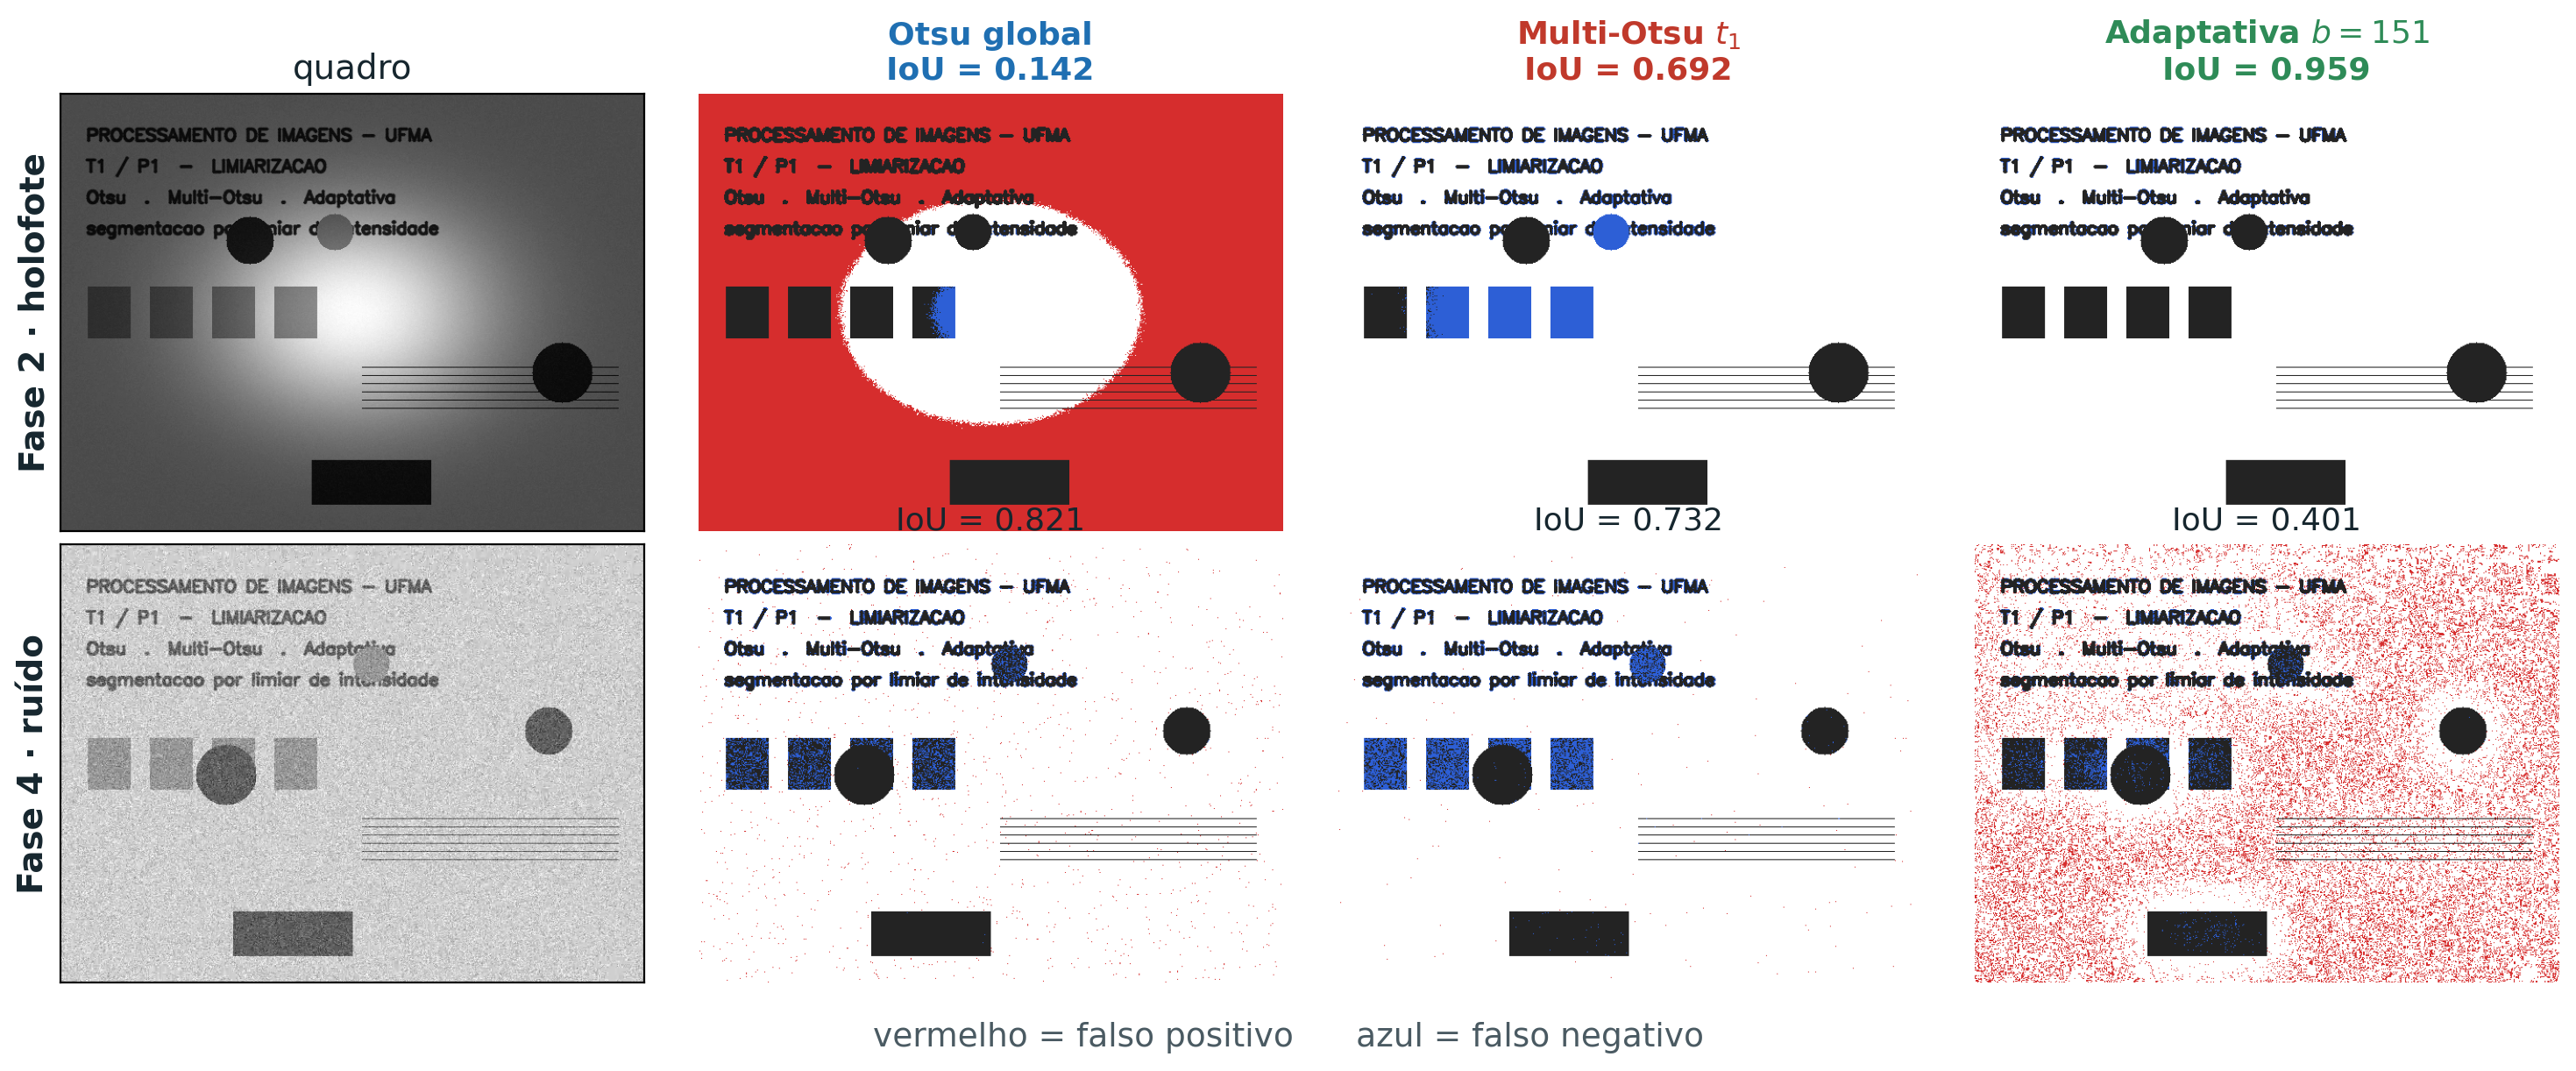
\includegraphics[width=.93\textwidth]{erros_slide}
  \end{center}

  \vspace{-.6em}
  \sub{No holofote, o Otsu pinta \textbf{70\,\%} da imagem de vermelho — declara
  objeto todo o fundo escurecido. Uma linha abaixo, com ruído, é a adaptativa
  que fica coberta de vermelho. \textbf{O pódio se inverte entre as duas
  linhas.}}

\end{frame}

% -----------------------------------------------------------------------------
\begin{frame}{A métrica que só aparece em vídeo}

  \begin{columns}[T,onlytextwidth]
    \column{.42\textwidth}
      \footnotesize
      \begin{tabular}{@{}lcc@{}}
        \toprule
        \textbf{Método} & \textbf{Fase 4} & \textbf{Global} \\
        \midrule
        Limiar fixo & 2,53\,\% & 1,67\,\% \\
        Otsu & 3,57\,\% & 1,48\,\% \\
        \textbf{Multi-Otsu $t_1$} & \textbf{1,81\,\%} & \textbf{0,66\,\%} \\
        Multi-Otsu $t_2$ & 19,38\,\% & 5,44\,\% \\
        Adaptativa $b{=}35$ & \textcolor{cMulti}{21,95\,\%} & 6,00\,\% \\
        Sauvola & 4,34\,\% & 1,58\,\% \\
        \bottomrule
      \end{tabular}

      \vspace{.8em}
      \normalsize
      \sub{Fração de pixels que trocam de classe entre quadros consecutivos.}

    \column{.54\textwidth}
      \vspace{1em}
      Na fase de ruído, a adaptativa faz \num{22\,\%} dos pixels
      \alert{piscarem} a cada quadro.

      \vspace{.8em}
      Visualmente insuportável, e fatal para qualquer etapa seguinte:
      rastreamento, contagem de objetos, OCR.

      \vspace{.8em}
      O Multi-Otsu $t_1$ é \textbf{12$\times$} mais estável.

      \vspace{.8em}
      \sub{Um método pode ter IoU aceitável e ainda assim ser inútil em vídeo.
      A análise de imagem estática jamais mostraria isso.}
  \end{columns}

\end{frame}

% -----------------------------------------------------------------------------
\begin{frame}{Custo: todos cabem em tempo real}

  \footnotesize
  \begin{center}
  \begin{tabular}{@{}lrrl@{}}
    \toprule
    \textbf{Método} & \textbf{ms/quadro} & \textbf{fps} & \\
    \midrule
    Otsu (OpenCV, C++)        & 0,16  & 6\,370 & \\
    Limiar fixo               & 0,34  & 2\,970 & \\
    Otsu (nossa implementação)& 0,88  & 1\,140 & \\
    Multi-Otsu $M=3$          & 1,20  & 830    & \\
    Sauvola                   & 3,73  & 268    & \\
    Adaptativa $b{=}35$       & 4,62  & 216    & \\
    \textbf{Adaptativa $b{=}151$} & \textbf{22,8} & \textbf{44} & folga pequena \\
    Multi-Otsu $M=4$ (skimage)& 32,8  & 31     & \textcolor{cMulti}{no limite} \\
    \bottomrule
  \end{tabular}
  \end{center}

  \vspace{.8em}
  \normalsize
  \sub{Quadros de 640$\times$480. A adaptativa pela \emph{média} com imagem
  integral é $O(N)$ independente de $b$ — se o custo incomodar, é ela que se
  usa, com a mesma robustez à iluminação.}

\end{frame}

% -----------------------------------------------------------------------------
\begin{frame}{Guia de escolha}

  \footnotesize
  \begin{center}
  \begin{tabular}{@{}E{.42\textwidth}E{.25\textwidth}E{.27\textwidth}@{}}
    \toprule
    \textbf{Situação} & \textbf{Método} & \textbf{Razão} \\
    \midrule
    Histograma bimodal, luz uniforme & \textcolor{cOtsu}{Otsu} & 0,944 em 0,88\,ms \\
    Brilho global varia (dia/noite, auto-exposição) & \textcolor{cOtsu}{Otsu} por quadro & invariante a mudança global \\
    Três ou mais populações, luz uniforme & \textcolor{cMulti}{Multi-Otsu $t_2$} & melhor global: 0,966 \\
    \textbf{Sombra, holofote, documento digitalizado} & \textcolor{cAdapt}{\textbf{Adaptativa}}, $b$ ajustado & único que segue $L(x,y)$ \\
    Objetos grandes e maciços & global, ou $b >$ objeto & senão esvazia o interior \\
    Ruído forte, baixo contraste & \textcolor{cOtsu}{global} ou \textcolor{cAdapt}{Sauvola} & média de $N$ cancela ruído \\
    Vídeo, estabilidade é crítica & \textcolor{cMulti}{Multi-Otsu $t_1$} & 0,66\,\% de cintilação \\
    Texto sobre fundo irregular & \textcolor{cAdapt}{Sauvola} & equilibra luz e ruído \\
    \bottomrule
  \end{tabular}
  \end{center}

\end{frame}

% =============================================================================
\section{Fechamento}

% -----------------------------------------------------------------------------
\begin{frame}{Três conclusões}

  \begin{enumerate}
    \setlength{\itemsep}{1.1em}
    \item O limiar global falha com variação \alert{espacial} de iluminação, não
      com variação temporal.
      \sub{O mesmo Otsu: 0,943 na fase 3, 0,139 na fase 2.}

    \item A limiarização adaptativa troca robustez à iluminação por fragilidade
      ao \alert{ruído}.
      \sub{Fase 2: 0,956. Fase 4: 0,575. As duas coisas têm a mesma causa —
      ela decide olhando poucos pixels.}

    \item \alert{Nenhum método venceu as quatro fases.}
      \sub{A escolha não é sobre qual técnica é melhor, e sim sobre qual
      hipótese a sua cena satisfaz.}
  \end{enumerate}

\end{frame}

% -----------------------------------------------------------------------------
\begin{frame}{O que ficou de fora}

  \begin{columns}[T,onlytextwidth]
    \column{.48\textwidth}
      \textbf{Limitações que assumimos}

      \vspace{.5em}
      \begin{itemize}
        \item O vídeo é sintético — escolha deliberada, para ter gabarito exato
          dos 600 quadros e isolar um fator por vez.
        \item Um único ajuste de parâmetros por método.
        \item Sem pós-processamento morfológico, que mudaria o ranking da
          fase 4.
      \end{itemize}

    \column{.48\textwidth}
      \textbf{Extensões naturais}

      \vspace{.5em}
      \begin{itemize}
        \item Pré-filtro gaussiano antes do Otsu — recomendação do próprio
          tutorial do OpenCV.
        \item Limiar com memória temporal:
          $T_k=\alpha T_{k-1}+(1-\alpha)T_k^{\text{Otsu}}$, para cortar a
          cintilação.
        \item Abertura morfológica após a adaptativa.
      \end{itemize}
  \end{columns}

\end{frame}

% -----------------------------------------------------------------------------
\begin{frame}[standout]
  Obrigado
  \vspace{.6em}

  {\small\normalfont Perguntas?}
\end{frame}

% -----------------------------------------------------------------------------
\begin{frame}[allowframebreaks]{Referências}

  \footnotesize
  \begin{thebibliography}{9}
    \bibitem{otsu}
      N.~Otsu. \emph{A Threshold Selection Method from Gray-Level Histograms}.
      IEEE Trans. SMC, 9(1):62--66, 1979.
    \bibitem{liao}
      P.-S.~Liao, T.-S.~Chen, P.-C.~Chung. \emph{A Fast Algorithm for Multilevel
      Thresholding}. J. Inf. Sci. Eng., 17:713--727, 2001.
    \bibitem{sauvola}
      J.~Sauvola, M.~Pietikäinen. \emph{Adaptive Document Image Binarization}.
      Pattern Recognition, 33(2):225--236, 2000.
    \bibitem{bradley}
      D.~Bradley, G.~Roth. \emph{Adaptive Thresholding using the Integral Image}.
      J. Graphics Tools, 12(2):13--21, 2007.
    \bibitem{sezgin}
      M.~Sezgin, B.~Sankur. \emph{Survey over image thresholding techniques and
      quantitative performance evaluation}. J. Electronic Imaging,
      13(1):146--165, 2004.
    \bibitem{gonzalez}
      R.~C.~Gonzalez, R.~E.~Woods. \emph{Digital Image Processing}, cap.~10.
    \bibitem{skimage}
      scikit-image. \texttt{plot\_thresholding} e \texttt{plot\_multiotsu}.
    \bibitem{opencv}
      OpenCV. \texttt{py\_thresholding} (Image Thresholding).
  \end{thebibliography}

\end{frame}

\end{document}
